\documentclass[journal]{IEEEtran}

\usepackage[OT1]{fontenc}
\usepackage{cite}
\usepackage{graphicx}
\usepackage{amsmath,amssymb}
\usepackage{booktabs}
\usepackage{multirow}
\usepackage{array}
\usepackage{url}
\usepackage[caption=false,font=footnotesize]{subfig}
\usepackage{algorithm}
\usepackage{algorithmic}
\usepackage{placeins}

\graphicspath{{figures/}}

% Avoid stacking multiple double-column floats
% at the top of the same page.
\setcounter{dbltopnumber}{1}
\renewcommand{\dbltopfraction}{0.85}
\renewcommand{\textfraction}{0.10}

\hyphenation{ap-prox-i-mate ac-cel-er-a-tor sur-ro-gate mul-ti-ob-jec-tive non-dom-i-nat-ed}

\title{ApproxPilot-SE: Co-Evolving Surrogate Models and DSE for Approximate Accelerators}

\author{Yanzhe~Wang,
        Cheng~Liu,
        Fangfa~Fu,
        Bing~Yang
        and~Jinxiang~Wang}

\begin{document}
\maketitle


\begin{abstract}
Approximate computing can reduce hardware cost with tolerable accuracy degradation, but finding high-quality designs under output-quality constraints still requires extensive design space exploration (DSE). Existing surrogate-assisted approaches typically rely on large training datasets constructed for the target accelerator or on pretrained models transferred from existing circuit domains.

This paper presents \emph{ApproxPilot-SE}, a co-evolving surrogate-assisted DSE framework for approximate accelerators under limited synthesis budgets. ApproxPilot-SE jointly optimizes approximation-site selection and arithmetic-unit assignment while iteratively selecting Pareto-relevant candidates for ground-truth evaluation. The newly measured power, performance, and area (PPA) and quality-of-result (QoR) labels are incorporated into subsequent surrogate updates, allowing surrogate learning and multi-objective search to progressively adapt to the regions exposed during optimization. With 900 target-system training labels on DCT76, ApproxPilot-SE achieves a verified 3-D PPA hypervolume (HV) gain of 0.085054 at 90\% structural similarity index (SSIM) retention, compared with 0.023273 for the stronger baseline at the same constraint. It also maintains a verified HV Gain of 0.067996 at 99\% retention, whereas both baselines provide no gain beyond the Exact reference. Under the same 900-label training budget, co-evolving optimization improves verified HV Gain over an aligned one-shot workflow by up to 50.84\%. A representative high-quality design retains 99.68\% of the Exact-design SSIM while reducing Area, Power, and Delay by 19.73\%, 20.50\%, and 12.71\%, respectively. These results show that coupling ground-truth feedback with surrogate-guided search can improve the quality of verified PPA--QoR tradeoffs under constrained target-system evaluation budgets.
\end{abstract}


\begin{IEEEkeywords}
approximate computing, design space exploration, graph neural networks, logic synthesis, surrogate modeling, electronic design automation.
\end{IEEEkeywords}

\section{Introduction}
\label{sec:introduction}

\IEEEPARstart{A}{pproximate}  computing trades bounded degradation in output quality for improvements in hardware area, power, and delay, providing an effective means of improving the efficiency of domain-specific accelerators~\cite{jiang2020approxarith,que2023approxsurvey,xu2016approxsurvey}. 
Approximate arithmetic libraries, such as EvoApprox8b~\cite{mrazek2017evoapprox}, provide diverse adders, subtractors, and multipliers with different error characteristics and hardware costs, enabling designers to construct approximate accelerators by selectively replacing exact arithmetic units.
However, when an accelerator contains many configurable arithmetic sites and each site admits multiple legal implementations, the number of system configurations grows combinatorially.
System-level power, performance, and area (PPA) depend on logic synthesis, structural interactions, and timing paths, so component costs alone do not determine the accelerator implementation.
Application quality is likewise determined by how local approximation errors propagate through the complete computation.
Consequently, exhaustive synthesis and application-level evaluation quickly become impractical, making efficient design space exploration (DSE) a central challenge in automated approximate-accelerator design~\cite{saeedi2024dse,silva2024mapping}.

Surrogate-assisted DSE has substantially reduced the cost of exploring such large spaces.
AutoAx~\cite{mrazek2019autoax} established an automated exploration methodology based on libraries of approximate components, while Xel-FPGAs~\cite{prabakaran2023xelfpgas} extended end-to-end automated exploration to FPGA-based approximate accelerators.
More recently, ApproxPilot~\cite{zhang2025approxpilot} introduced graph-neural-network-based modeling for accelerator approximation, and ApproxGNN~\cite{vlcek2025approxgnn} explored pretrained graph representations for parameter prediction in approximate-computing DSE.
These advances demonstrate that learned surrogates can replace a large fraction of expensive hardware evaluations and enable exploration of design spaces that would otherwise be difficult to search directly.

The central challenge is to align surrogate learning with the regions that matter to optimization.
Multi-objective DSE does not query the design space uniformly.
As optimization progresses, the search increasingly concentrates on configurations that appear competitive with respect to the current Pareto front.
Therefore, prediction quality in these Pareto-relevant regions is more important to the final optimization outcome than uniformly high accuracy over the entire design space.
In representative surrogate-based approximate-accelerator flows, the surrogate is trained or adapted before the main search and is subsequently used to evaluate a much larger set of candidate configurations~\cite{mrazek2019autoax,zhang2025approxpilot,vlcek2025approxgnn}.
Evaluating promising configurations identified during DSE provides system-level supervision directly relevant to subsequent search.
Feedback-driven evaluation has already proved useful for other expensive hardware optimization problems, including Bayesian and active-learning-based DSE~\cite{reagen2017bayesopt,bai2021boomexplorer,huang2024arsflow,huang2025arsflow2}.
For approximate accelerators, the key question is how to couple such feedback with simultaneous PPA and application-quality modeling over a large, heterogeneous, multi-site approximation space.

Delay modeling poses a second challenge because its structural dependence differs from that of area and power.
While area and power reflect aggregate effects across the synthesized design, system delay is dominated by dependencies along competing combinational paths.
ApproxPilot explicitly incorporates critical-path information into its delay modeling~\cite{zhang2025approxpilot}.
More broadly, graph-based delay prediction has demonstrated the importance of structural information in both FPGA and ASIC-oriented modeling~\cite{ustun2020delay,de2023asicdelay}.
Motivated by this property, we directly propagate and aggregate latent node representations along RTL timing domains and directed dependencies.
The resulting representation captures path-dependent delay behavior at the configuration level without requiring explicit critical-path node labels.

We present \textbf{ApproxPilot-SE}, an extension of ApproxPilot that couples surrogate learning and DSE through iterative ground-truth feedback.
Separate PPA and quality-of-result (QoR) surrogates guide the search over legal configurations of the target accelerator.
Non-dominated sorting and crowding distance identify Pareto-relevant candidates for logic synthesis and application-level evaluation.
The measured labels update both surrogates, directing subsequent search toward regions informed by the new measurements.
After the iterative search terminates, the final candidate set is evaluated using logic synthesis and application-level quality measurement to construct the verified Pareto front.

The main contributions of this work are summarized as follows:

\begin{itemize}

    \item \textbf{A co-evolving PPA--QoR DSE framework for multi-site approximate-accelerator optimization.}
    ApproxPilot-SE couples multi-objective search with iterative system-level feedback: Pareto-relevant configurations identified during DSE are evaluated for real PPA and QoR, incorporated into the training set, and used to update both surrogates before the next search round.
    Under the same 900-label target-system training budget, ApproxPilot-SE improves ground-truth hypervolume (HV) gain over an aligned one-shot workflow by \textbf{50.84\%} at 99\% SSIM retention on DCT76.

    \item \textbf{A timing-domain path aggregation mechanism without explicit critical-path node supervision.}
    ApproxPilot-SE propagates latent node representations along directed RTL dependencies within timing domains and aggregates competing paths into a structure-aware representation for system-level delay prediction.
    Across three paired training seeds, the proposed readout reduces Delay MAE by \textbf{7.45\%} relative to global max pooling, while improving Spearman correlation from \textbf{0.7965} to \textbf{0.8217} and pairwise ranking accuracy from \textbf{80.37\%} to \textbf{81.67\%}.

    \item \textbf{An end-to-end, ground-truth-verified optimization flow for approximate accelerators.}
    ApproxPilot-SE integrates legal configuration generation, PPA/QoR modeling, co-evolving search, and final synthesis- and application-level verification into a unified system-level workflow.
    On DCT76, it achieves higher ground-truth PPA HV gain than ApproxPilot and ApproxGNN under all five SSIM-retention constraints from 80\% to 99\%.
    A representative high-quality design retains \textbf{99.68\%} of the Exact SSIM while reducing Area, Power, and Delay by \textbf{19.73\%}, \textbf{20.50\%}, and \textbf{12.71\%}, respectively.

\end{itemize}

The remainder of this paper is organized as follows.
Section~\ref{sec:related} reviews automated approximate-accelerator design, learning-based hardware modeling, and sequential DSE with expensive evaluations.
Section~\ref{sec:method} presents the surrogate models, timing-domain path aggregation, and the co-evolution of surrogate learning and DSE in ApproxPilot-SE.
Section~\ref{sec:experiments} evaluates ApproxPilot-SE in terms of ground-truth Pareto quality, surrogate ranking quality, the effect of co-evolving optimization, delay modeling, and representative hardware designs.
Section~\ref{sec:conclusion} concludes the paper.

\section{Related Work}
\label{sec:related}

\subsection{Automated Approximate-Accelerator Design}

Approximate computing has produced a broad range of circuit-, architecture-, and system-level techniques for trading output accuracy against hardware efficiency \cite{xu2016approxsurvey}. Recent surveys of approximate-computing DSE further show that automated exploration commonly combines arithmetic approximation with evolutionary, learning-based, or search-based optimization \cite{saeedi2024dse,silva2024mapping}. Approximate arithmetic libraries such as EvoApproxLib and related collections provide large sets of implementations with different error and hardware characteristics \cite{mrazek2017evoapprox,hanif2017quad,ullah2018smapproxlib}.

Automation has been studied at several abstraction levels. Approximate logic synthesis directly transforms Boolean or gate-level implementations under explicit error constraints \cite{miao2013als,venkataramani2020logicsynthesis}. Axilog provides language-level support for identifying relaxable portions of RTL hardware \cite{yazdanbakhsh2015axilog}, while Chisel selects approximate operations according to application-level reliability and accuracy constraints \cite{misailovic2014chisel}. These studies establish approximation placement as an important design decision in automated approximate computing.

At the accelerator level, ABACUS, AutoAx, and AxHLS automate the construction of larger approximate systems from approximate operations or components \cite{nepal2014abacus,mrazek2019autoax,castrogodinez2020axhls}. FPGA-oriented and multi-stage frameworks further extend automated approximate design across different implementation flows \cite{prabakaran2020approxfpgas,prabakaran2023xelfpgas,meng2023hedals,meng2025appresub}. Search-based approaches have also been introduced to navigate large approximate design spaces, including Monte-Carlo-tree-search-based accelerator synthesis and learning-assisted approximate-circuit DSE \cite{awais2021mcts,awais2021ldax}.

A common accelerator-level formulation assigns one library implementation to each operation exposed to DSE. AutoAx represents an accelerator configuration through approximate-component assignments \cite{mrazek2019autoax}, and ApproxPilot similarly optimizes arithmetic-unit choices across accelerator operations \cite{zhang2025approxpilot}. For large RTL targets, approximation placement and unit assignment become closely coupled because the most effective design may retain Exact implementations at a substantial subset of legally configurable sites. This motivates a search space in which Exact and approximate implementations are treated uniformly as candidate states at each configurable arithmetic operation.

\subsection{Learning-Based PPA/QoR Modeling and Transfer}

Machine learning has become an established means of reducing repeated EDA evaluations, spanning performance prediction, physical-design estimation, black-box optimization, and learned circuit representations \cite{huang2021mleda}. GNN-based EDA further exploits the natural graph structure of RTL, netlists, and circuit data \cite{sanchez2023gnneda}.

For high-level and accelerator design, graph models have been applied to latency and performance estimation and to learning-assisted design-space exploration \cite{ustun2020delay,wu2022hls_gnn,wu2023ironmanpro}. Related models address power and PPA prediction \cite{lin2022powergear,lin2023hlpow,zhao2025pdnnet}, while structural circuit representation learning provides reusable graph embeddings for downstream EDA tasks \cite{xu2022sns,li2022deepgate,shi2023deepgate2}.

Learning-based modeling has also become central to approximate-accelerator exploration. AutoAx uses conventional regression models to estimate accelerator-level hardware cost and output quality \cite{mrazek2019autoax}. ApproxPilot introduces graph-based models together with critical-path-aware delay prediction \cite{zhang2025approxpilot}. These methods construct target-specific prediction models from sampled accelerator configurations.

ApproxGNN develops a complementary transfer-oriented approach. It learns approximate-component embeddings from a reusable corpus of 15.9K configurations generated from 159 random image-convolution kernels and evaluates transfer to unseen Small and Large Gaussian filters \cite{vlcek2025approxgnn}. This demonstrates that learned component representations can be reused across related accelerator structures and reduces the need to train every predictor entirely from scratch.

Unit characterization provides another reusable source of information. Area, Power, Delay, and error properties of arithmetic units can be obtained independently of a particular accelerator and incorporated into its graph representation. The resulting system model can use target-system labels to capture composition, synthesis, and topology-dependent interactions while retaining reusable local hardware information.

\subsection{Sequential Optimization with Expensive Evaluations}

Design-space exploration under expensive evaluation budgets has been widely studied using surrogate and sequential optimization. Bayesian optimization provides a general framework for choosing new evaluations from the current predictive model \cite{shahriari2016bo,knowles2006parego,wang2023bo}, while trust-region and tree-based approaches extend model-based optimization to larger and more structured spaces \cite{eriksson2019turbo,wang2020lamcts,zhao2021mopartitions}.

Sample-efficient optimization has also been applied directly to hardware design. HyperMapper supports multiobjective design-space exploration with expensive and potentially infeasible evaluations and has been demonstrated on hardware accelerator tuning \cite{nardi2019hypermapper}. BOOM-Explorer combines active sampling, learned surrogate modeling, and multiobjective Bayesian optimization for processor microarchitecture DSE \cite{bai2021boomexplorer}. Accelerator-rich systems have similarly been explored with active-learning-based refinement around promising Pareto regions in ARS-Flow and its extended formulation ARS-Flow 2.0 \cite{huang2024arsflow,huang2025arsflow2}.

Related ideas appear in accelerator design, approximate arithmetic, circuit optimization, and Pareto-front identification. Bayesian optimization has been applied to accelerator DSE \cite{reagen2017bayesopt}, while active or surrogate-guided methods have been investigated for approximate adders and circuit design \cite{ma2019adder_active,ma2019cadbo}. Other work considers surrogate-assisted multiobjective search, Pareto identification, and active evaluation in hardware and circuit optimization \cite{geng2022gnp,belwal2022qpir,cao2025roseopt,chen2026yield,yin2022activeyield}.

These methods establish the value of allocating expensive evaluations according to an evolving optimization state. Approximate-accelerator DSE adds a distinctive coupling between this allocation problem and the underlying configuration space: the optimizer must simultaneously determine approximation placement, arithmetic-unit binding, and which target-system configurations should receive the next synthesis evaluations. ApproxPilot-SE integrates these decisions within a single closed-loop DSE process under a fixed target-specific evaluation budget.
\section{ApproxPilot-SE Methodology}
\label{sec:method}

ApproxPilot-SE targets system-level design space exploration for approximate accelerators with multiple configurable arithmetic sites. Given a target RTL design and a pre-characterized approximate arithmetic-unit library, the framework constructs a legal configuration space, represents each candidate over the shared RTL topology, and estimates its hardware cost and application quality using learned PPA and QoR surrogates. The overall framework is illustrated in Fig.~\ref{fig:framework}.

A central feature of ApproxPilot-SE is that surrogate learning and design space exploration are coupled rather than treated as two isolated stages. The current surrogates guide the search toward competitive regions of the design space, while Pareto-relevant candidates are selected for ground-truth logic synthesis and application-level evaluation. Their measured PPA and QoR values are then incorporated into the training set to update the surrogates before the next search round. In this way, the search determines where new measurements are collected, and the resulting measurements reshape the models that drive subsequent exploration. After the iterative process, the updated surrogates support a larger final search, whose selected candidates are evaluated using ground-truth system-level measurements to construct the reported Pareto front.

\begin{figure*}[t]
    \centering
    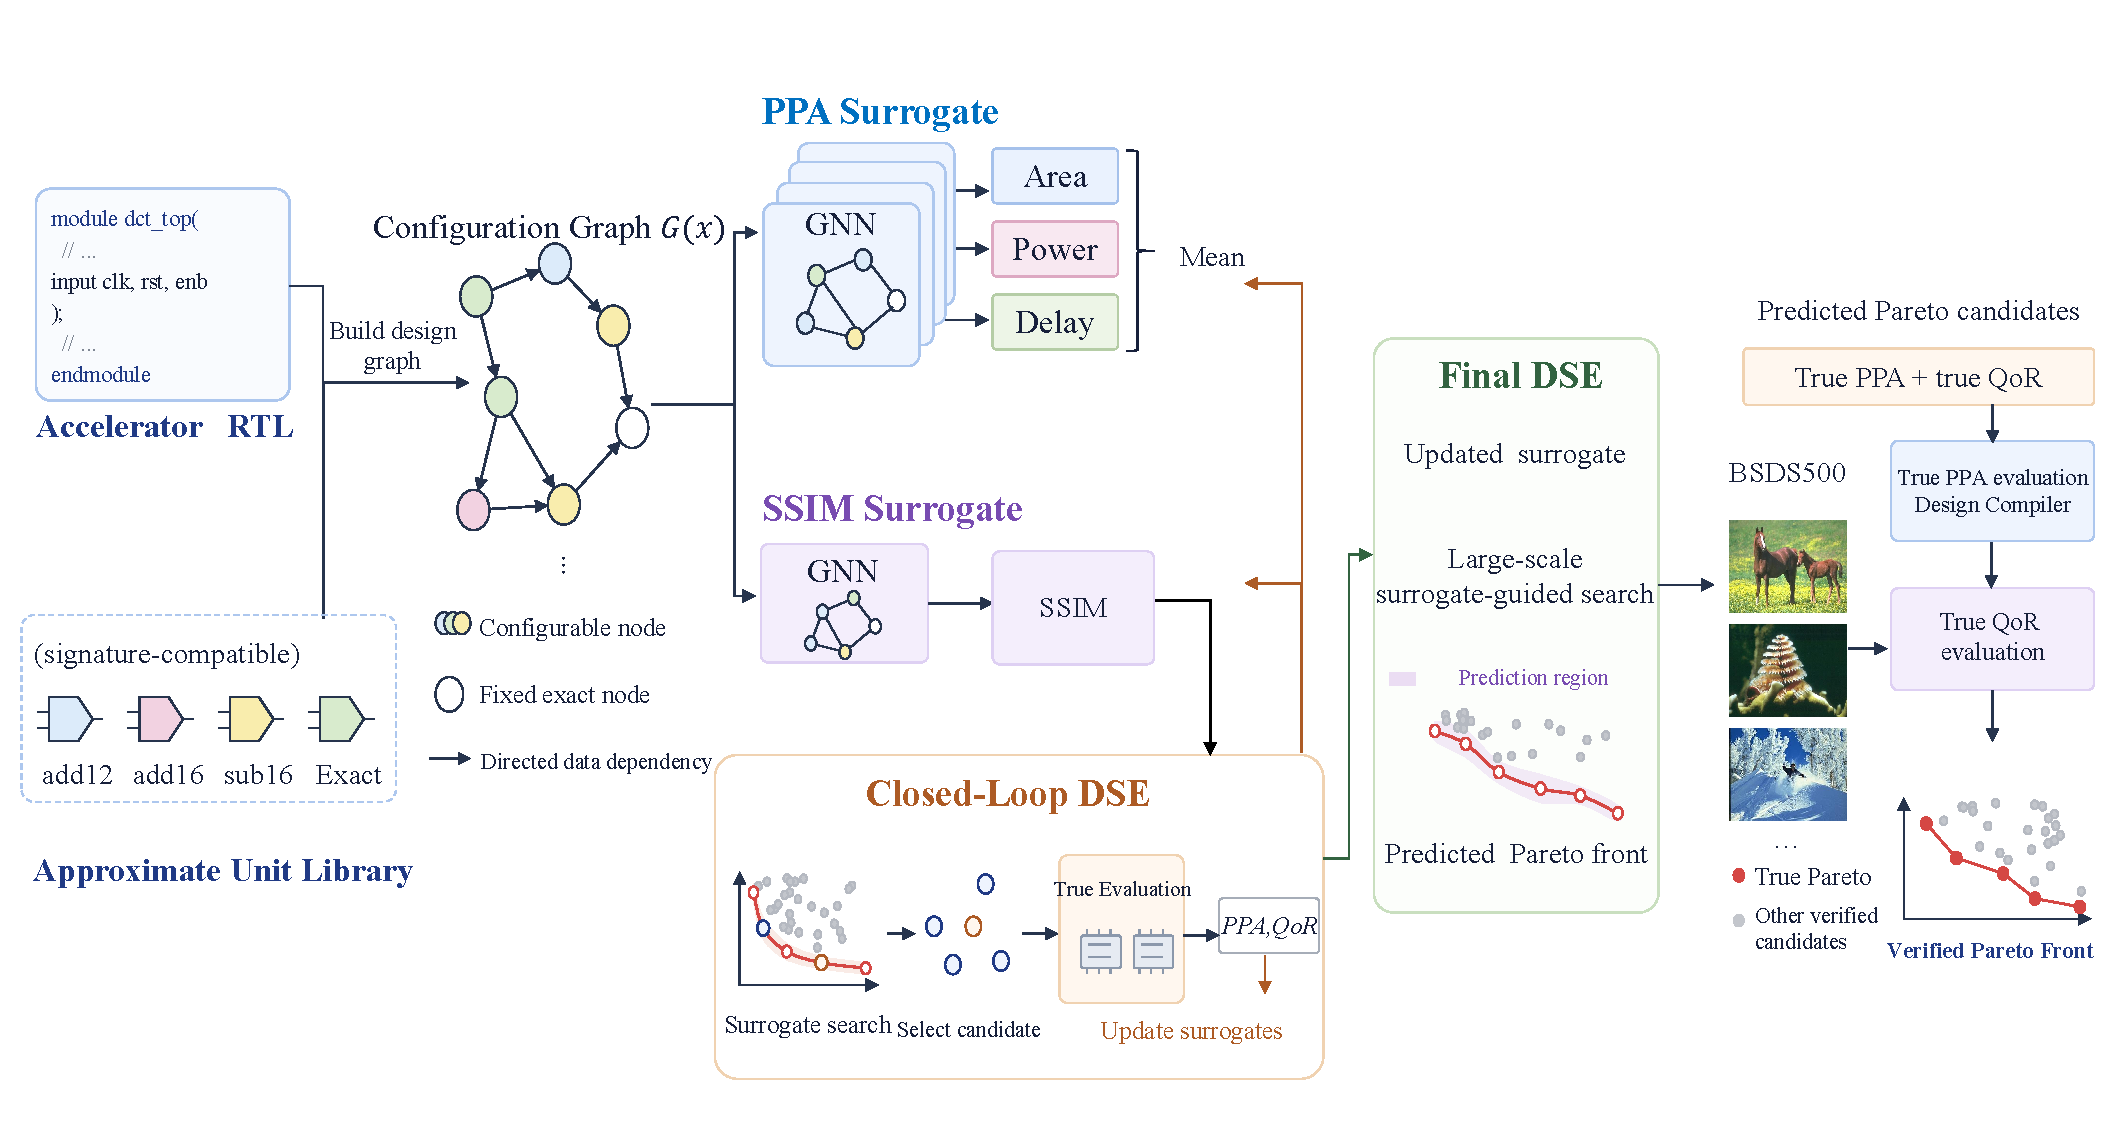
\includegraphics[width=0.98\textwidth]{figures/framework_v4.pdf}
    \caption{Overview of ApproxPilot-SE. Candidate accelerator configurations are represented on the RTL graph and evaluated by PPA and QoR surrogates. Pareto-relevant candidates identified during DSE receive ground-truth PPA and QoR evaluations, and the resulting labels are used to update the surrogate models for subsequent search rounds. The final Pareto front is reconstructed exclusively from ground-truth system-level evaluations.}
    \label{fig:framework}
\end{figure*}

ApproxPilot-SE consists of three closely connected components: configuration-aware graph modeling, system-level PPA and QoR surrogate prediction, and co-evolving surrogate-assisted DSE. The following subsections describe these components, with particular emphasis on the timing-domain path aggregation used for Delay modeling and the iterative interaction between surrogate learning and search.


\subsection{Configuration Space and Graph Representation}
\label{sec:configuration_graph}

The design space of ApproxPilot-SE is defined directly over the legal implementations of the configurable arithmetic sites in the target RTL. This formulation provides a unified representation for Exact and Approximate implementations while preserving the structural context in which each implementation operates.

Let
\begin{equation}
    \mathcal{V}_{\mathrm{cfg}}=\{1,2,\ldots,N\}
\end{equation}
denote the set of configurable arithmetic sites in the target accelerator. For site $i$, let $e_i$ denote its exact implementation and $\mathcal{A}_i$ the set of approximate arithmetic units compatible with its RTL interface. The legal implementation set of site $i$ is therefore defined as
\begin{equation}
    \mathcal{C}_i=\{e_i\}\cup\mathcal{A}_i .
    \label{eq:site_state}
\end{equation}
A complete accelerator configuration is represented by
\begin{equation}
    \mathbf{x}=[x_1,x_2,\ldots,x_N],
    \qquad
    x_i\in\mathcal{C}_i .
    \label{eq:configuration}
\end{equation}

This formulation places Exact and Approximate implementations in the same discrete configuration space. Selecting $e_i$ keeps site $i$ exact, whereas selecting an element of $\mathcal{A}_i$ assigns the corresponding approximate arithmetic unit. The candidate set may differ across sites because legality is determined by the operation type, signedness, and input/output interfaces of the original RTL operator. Arithmetic nodes that are structurally fixed to Exact implementations are excluded from the design variables but remain in the complete RTL graph, thereby preserving the original data dependencies.

For a configuration $\mathbf{x}$, its ground-truth system response is defined as
\begin{equation}
    \mathbf{y}(\mathbf{x})
    =
    \left[
    A(\mathbf{x}),
    P(\mathbf{x}),
    D(\mathbf{x}),
    Q(\mathbf{x})
    \right],
    \label{eq:system_response}
\end{equation}
where $A(\mathbf{x})$, $P(\mathbf{x})$, and $D(\mathbf{x})$ denote post-synthesis Area, Power, and Delay, respectively, and $Q(\mathbf{x})$ denotes application-level quality of result (QoR). Using the fully exact accelerator as the hardware reference, the multi-objective search operates on
\begin{equation}
    \mathbf{f}(\mathbf{x})
    =
    \left[
    \frac{A(\mathbf{x})}{A_{\mathrm{ex}}},
    \frac{P(\mathbf{x})}{P_{\mathrm{ex}}},
    \frac{D(\mathbf{x})}{D_{\mathrm{ex}}},
    1-Q(\mathbf{x})
    \right].
    \label{eq:objectives}
\end{equation}
The optimization therefore seeks nondominated accelerator configurations that balance application quality against system-level hardware cost, rather than optimizing the local characteristics of individual approximate units in isolation.

To model the system-level behavior induced by different configurations, ApproxPilot-SE represents the target accelerator as a directed graph
\begin{equation}
    G(\mathbf{x})=(V,E,\mathbf{X}(\mathbf{x})),
    \label{eq:graph}
\end{equation}
where $V$ contains arithmetic-operation nodes, $E$ captures directed RTL data dependencies, and $\mathbf{X}(\mathbf{x})$ denotes configuration-dependent node attributes. Candidate configurations of the same accelerator share the underlying RTL topology, while the implementation assigned to each configurable node and its associated attributes vary with $\mathbf{x}$. This representation allows the surrogate models to distinguish different Exact/Approximate assignments while retaining the structural context in which those assignments affect the complete accelerator.

Each node representation combines two complementary types of information. The first characterizes the RTL operator and its structural context, including operation and interface attributes as well as its position in the directed dataflow graph. The second characterizes the implementation selected by the current configuration, including unit-level hardware properties and numerical-error descriptors. These local descriptors capture the behavior of individual arithmetic implementations, whereas their system-level effects are learned over the complete RTL graph rather than approximated by directly accumulating unit-level metrics.

The resulting configuration-aware graph provides a common structural basis for the PPA and QoR surrogates. The PPA branch learns how local implementation choices interact through the RTL topology to determine Area, Power, and Delay, whereas the QoR branch additionally exploits approximation-error characteristics to capture their impact on application-level quality. The two surrogate models are described next.





% B PPA 与 QoR 代理模型
\subsection{PPA and QoR Surrogate Models}
\label{sec:surrogate_models}

ApproxPilot-SE employs separate PPA and QoR surrogates to rapidly evaluate the hardware cost and application quality of candidate configurations. For a given accelerator, the RTL data-dependency topology remains fixed, while the attributes of configurable nodes change with the selected Exact or Approximate implementations. The surrogates therefore learn how different arithmetic-unit assignments translate into system-level behavior over the same underlying computation graph.

The PPA surrogate uses a four-layer directed graph encoder with 128-dimensional hidden representations. Each node is initialized from its RTL attributes, structural information, and the characteristics of the currently selected arithmetic implementation. Information is then propagated along directed RTL dependencies so that the resulting node representation captures both the local implementation and its upstream computation context.

Area and Power are predicted using two independent learned graph readouts. Each readout assigns objective-specific importance to the encoded nodes, forming a graph-level representation tailored to the corresponding hardware metric. This representation is combined with configuration-level global features and passed to an independent regression head to estimate post-synthesis Area or Power. Unit-level physical characteristics describe the local implementations, while their system-level effects are learned from the complete accelerator graph rather than obtained by directly accumulating individual unit costs.

Delay shares the same directed graph encoder but uses a different readout. Because system delay is strongly shaped by directed data paths and competition among them, ApproxPilot-SE preserves path structure when constructing the Delay representation instead of relying on conventional global aggregation. The resulting timing-domain path aggregation is described in Section~\ref{sec:path_aggregation}.

The QoR surrogate is implemented as a separate five-layer GraphSAGE model with 128-dimensional hidden representations. In addition to RTL and configuration information, its node features include numerical-error descriptors of the selected arithmetic units. The encoded node representations are jointly used to predict the quality response for multiple application inputs, whose mean serves as the configuration-level QoR used during DSE. This model directly captures the mapping from arithmetic-unit assignments to application-level output quality over the complete computation graph.

PPA and QoR prediction use ensembles of five and three independently trained models, respectively, with the ensemble mean serving as the surrogate estimate during search. For a candidate configuration $\mathbf{x}$, the two branches jointly provide
\begin{equation}
    \left[
    \hat{A}(\mathbf{x}),
    \hat{P}(\mathbf{x}),
    \hat{D}(\mathbf{x}),
    \hat{Q}(\mathbf{x})
    \right],
\end{equation}
enabling efficient system-level evaluation of a large number of candidate designs during multi-objective DSE.






% C 时序域路径聚合

\subsection{Timing-Domain Path Aggregation}
\label{sec:path_aggregation}

System Delay is governed by the propagation of signals along directed computation paths. The timing impact of an arithmetic implementation therefore depends on both its local characteristics and its position within the RTL dataflow. ApproxPilot-SE incorporates this path dependency through a timing-domain readout built on the node representations produced by the directed graph encoder.

Let $\mathbf{h}_v$ denote the encoded representation of node $v$. Within each timing domain, node states are propagated in topological order so that information accumulated along upstream paths is retained. For node $v$ in timing domain $d$, let $\mathrm{Pred}_d(v)$ denote its in-domain predecessors. The path state is defined as

\begin{equation}
    \mathbf{z}_{d,v}
    =
    \mathbf{h}_v
    +
    \max_{u\in\mathrm{Pred}_d(v)}
    \mathbf{z}_{d,u},
    \label{eq:path_recurrence}
\end{equation}

where the maximum is taken element-wise over the feature dimensions. For a source node within the timing domain,

\begin{equation}
    \mathbf{z}_{d,v}=\mathbf{h}_v .
    \label{eq:path_source}
\end{equation}

This recurrence accumulates node information along directed paths while retaining the strongest responses when multiple predecessor paths converge. Processing nodes in topological order allows each path state to summarize the implementation and structural information propagated from its upstream computation.

The resulting states are aggregated within each timing domain and then across timing domains:

\begin{equation}
    \mathbf{r}_D
    =
    \max_d
    \left(
        \max_{v\in V_d}
        \mathbf{z}_{d,v}
    \right),
    \label{eq:delay_readout}
\end{equation}

where $V_d$ denotes the nodes belonging to timing domain $d$. The resulting representation is combined with the configuration-level global features and mapped to the system-level Delay prediction:

\begin{equation}
    \hat{D}(\mathbf{x})
    =
    f_D
    \left(
        [\mathbf{r}_D \Vert \mathbf{g}(\mathbf{x})]
    \right).
    \label{eq:delay_prediction}
\end{equation}

The path recurrence operates on GNN-encoded node representations, while the final mapping to Delay is learned directly from system-level Delay labels. Consequently, the model incorporates RTL path order and path competition without requiring explicit critical-path node labels. The resulting path-aware representation provides the Delay surrogate used by ApproxPilot-SE during design space exploration.









% D 代理模型与 DSE 的协同演化
\subsection{Co-Evolving Surrogates and DSE}
\label{sec:coevolving_dse}

ApproxPilot-SE couples surrogate learning with multi-objective DSE through iterative ground-truth feedback. Let $\mathcal{D}_r$ denote the labeled set available at the beginning of round $r$. The PPA and QoR surrogates are trained on $\mathcal{D}_r$ and used to evaluate a large number of candidate configurations during search. Pareto-relevant candidates identified by the current search are then evaluated at the system level, and the resulting measurements are incorporated into the labeled set before the next round.

At round $r$, the current surrogates provide
\begin{equation}
    \left[
    \hat{A}_r(\mathbf{x}),
    \hat{P}_r(\mathbf{x}),
    \hat{D}_r(\mathbf{x}),
    \hat{Q}_r(\mathbf{x})
    \right]
\end{equation}
for each candidate configuration $\mathbf{x}$. ApproxPilot-SE uses these predictions to drive an NSGA-III search~\cite{deb2014nsga3} over the legal configuration space. Previously evaluated configurations are excluded from acquisition, and the remaining candidates are ranked by predicted nondominated fronts over the four objectives. Candidates are selected front by front so that ground-truth evaluations are concentrated on configurations with high optimization relevance.

When the remaining acquisition budget cannot accommodate an entire front, crowding distance~\cite{deb2002nsga2} is used to select candidates from that front. A larger crowding distance indicates a sparser neighborhood in the objective space; prioritizing such candidates preserves diverse PPA--QoR tradeoffs within the same nondomination level. The selected batch at round $r$ is denoted by $\mathcal{B}_r$.

Each configuration in $\mathcal{B}_r$ is then evaluated using logic synthesis and application-level execution to obtain
\begin{equation}
    \mathbf{y}(\mathbf{x})
    =
    \left[
    A(\mathbf{x}),
    P(\mathbf{x}),
    D(\mathbf{x}),
    Q(\mathbf{x})
    \right],
    \qquad
    \mathbf{x}\in\mathcal{B}_r .
\end{equation}
The newly measured configurations are added to the labeled set as
\begin{equation}
    \mathcal{D}_{r+1}
    =
    \mathcal{D}_{r}
    \cup
    \left\{
    (\mathbf{x},\mathbf{y}(\mathbf{x}))
    \mid
    \mathbf{x}\in\mathcal{B}_r
    \right\}.
    \label{eq:data_update}
\end{equation}

Both the PPA and QoR surrogates are retrained on $\mathcal{D}_{r+1}$ and immediately used in the next round of DSE. The search therefore determines where new ground-truth measurements are collected, while the newly acquired measurements reshape the surrogates that guide subsequent exploration. This bidirectional interaction constitutes the co-evolution of surrogate models and DSE in ApproxPilot-SE.

After the feedback rounds, the updated surrogates are used for a larger final search. A final set of Pareto-relevant candidates is selected from the predicted archive and evaluated using the same ground-truth PPA and QoR flow. The reported Pareto front is then reconstructed from the measured final candidates together with the Exact reference design. Surrogates determine where the design space is explored, whereas the reported hardware tradeoffs are determined by ground-truth system-level evaluations.

Algorithm~\ref{alg:coevolving} summarizes the complete procedure.

\begin{algorithm}[t]
\caption{Co-Evolving Surrogate Models and DSE in ApproxPilot-SE}
\label{alg:coevolving}
\begin{algorithmic}[1]
\REQUIRE legal design space $\Omega$, initial labeled set $\mathcal{D}_0$,
         feedback rounds $R$, acquisition budgets $\{B_r\}_{r=0}^{R-1}$,
         final candidate budget $B_f$
\STATE train the PPA and QoR surrogates on $\mathcal{D}_0$
\FOR{$r=0$ to $R-1$}
    \STATE run NSGA-III over $\Omega$ using the current surrogate objectives
    \STATE remove previously evaluated configurations
    \STATE rank the remaining candidates by predicted nondominated fronts
    \STATE select $B_r$ candidates using front order and crowding distance
    \STATE obtain ground-truth PPA and QoR for the selected candidates
    \STATE update $\mathcal{D}_{r+1}$ with the new measurements
    \STATE retrain the PPA and QoR surrogates on $\mathcal{D}_{r+1}$
\ENDFOR
\STATE perform the final surrogate-assisted search
\STATE select $B_f$ final candidates
\STATE obtain ground-truth PPA and QoR for all final candidates
\STATE reconstruct the Pareto set from the measured final candidates and Exact
\RETURN ground-truth nondominated set
\end{algorithmic}
\end{algorithm}

%\FloatBarrier
\section{Experimental Evaluation}
\label{sec:experiments}

\subsection{Experimental Setup}
\label{sec:setup}





\begin{figure*}[!t]
    \centering
    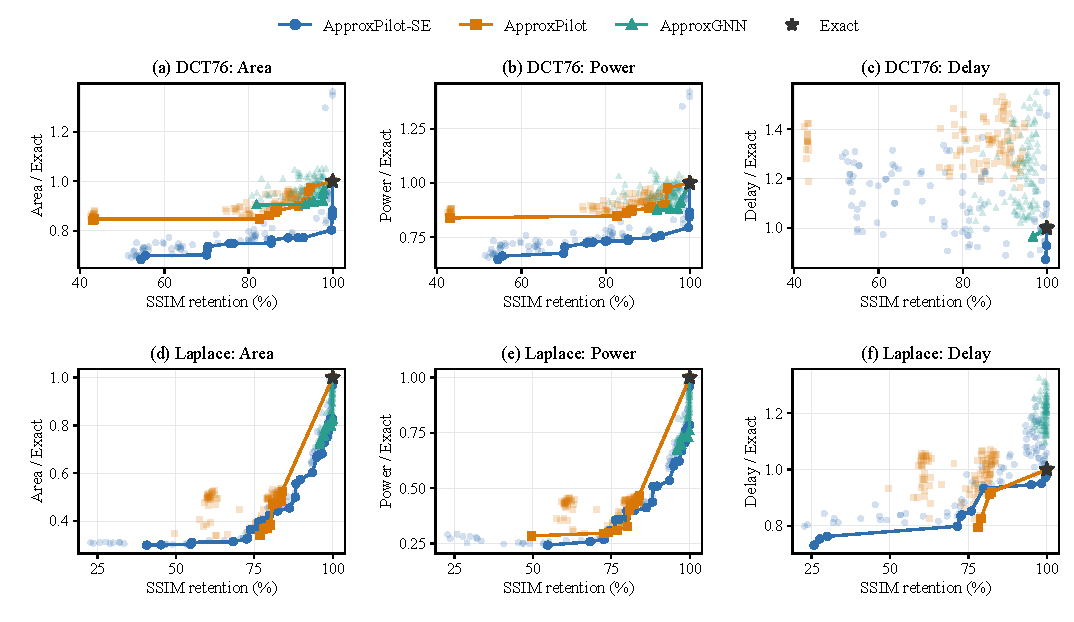
\includegraphics[width=\textwidth]{figures/measured_pareto.pdf}
    \caption{Measured PPA--QoR tradeoffs on DCT76 and Laplace.
    All plotted points correspond to final candidate designs evaluated
    using logic synthesis and application-level QoR evaluation.
    Faint markers show measured candidates, and connected markers show
    the two-dimensional nondominated fronts. Stars indicate the Exact designs.}
    \label{fig:measured_pareto}
\end{figure*}




Five approximate-accelerator benchmarks are considered: DCT, Laplace, Sobel, Gaussian, and KMeans, covering different arithmetic compositions and design-space sizes. For each benchmark, the legal Exact/Approximate configuration space is constructed according to the arithmetic operations and RTL interfaces of the target design. Table~\ref{tab:benchmarks} summarizes the benchmark characteristics.

\begin{table}[t]
\centering
\caption{Summary of the evaluated approximate-accelerator benchmarks.}
\label{tab:benchmarks}
\footnotesize
\setlength{\tabcolsep}{5pt}
\begin{tabular}{lcc}
\toprule
Benchmark & Arithmetic Operations & Configurable Sites \\
\midrule
DCT      & Add / Sub               & 76 \\
Laplace  & Add                     & 60 \\
Sobel    & Add / Sub               & 5  \\
Gaussian & Add / Mul               & 17 \\
KMeans   & Add / Sub / Mul / Sqrt  & 16 \\
\bottomrule
\end{tabular}
\end{table}

Candidate designs are synthesized using Synopsys Design Compiler with the FreePDK45 45-nm standard-cell library, from which system-level Area, Power, and Delay are obtained. Application quality is evaluated on BSDS500 images~\cite{arbelaez2011contour} using the structural similarity index (SSIM)~\cite{wang2004ssim}. DCT76 uses eight grayscale images, with SSIM measured between the reconstructed output and the input image. SSIM retention is the ratio of a candidate's mean SSIM to that of the corresponding Exact design. Final PPA and QoR results are obtained from logic synthesis and application execution.

ApproxPilot-SE is compared with ApproxPilot and ApproxGNN. Each method retains its own surrogate and search strategy over the same legal configuration space and system-level evaluation flow. On DCT76, each method uses 900 training configurations, a common 60-configuration validation set, and 15,000 final search trials with seed 101. Each final archive contains 100 measured candidates and Exact; training and validation configurations are excluded. ApproxPilot retains its critical-path supervision, and ApproxGNN uses its official pretrained component embeddings. DCT76 is also used to analyze co-evolving DSE, surrogate ranking quality, and Delay modeling.

Area, Power, and Delay are normalized to the Exact design of each benchmark. PPA tradeoffs are evaluated under SSIM-retention constraints of 80\%, 85\%, 90\%, 95\%, and 99\%, and three-dimensional hypervolume (HV) is used to quantify the Pareto region satisfying each quality constraint. The additional tradeoff space beyond the Exact design is reported as HV Gain:

\begin{equation}
    \mathrm{HV}_{\mathrm{gain}}
    =
    \mathrm{HV}
    \left(
        \mathcal{S}\cup\{\mathrm{Exact}\};\mathbf{r}
    \right)
    -
    \mathrm{HV}
    \left(
        \{\mathrm{Exact}\};\mathbf{r}
    \right),
    \label{eq:hv_gain}
\end{equation}

where $\mathcal{S}$ denotes the set of measured candidates satisfying the corresponding SSIM-retention constraint, and $\mathbf{r}=(1.10,1.10,1.70)$ is the reference point in the normalized PPA space. The same normalization and metric definitions are applied to all methods within each benchmark.
























\subsection{Design Space Exploration}
\label{sec:dse_results}

We evaluate the end-to-end optimization quality of
ApproxPilot-SE against ApproxPilot and ApproxGNN using
measured PPA--QoR tradeoffs and quality-constrained HV Gain.



Fig.~\ref{fig:measured_pareto} presents the measured PPA--QoR
tradeoffs on DCT76 and Laplace. Each point corresponds to a
final candidate evaluated using the complete ground-truth flow.
The projected fronts provide a direct view of how the three
methods distribute verified designs across different hardware-cost
and output-quality regions.

On DCT76, ApproxPilot-SE maintains verified PPA improvements
over a broad range of SSIM retention. Its candidates extend the
measured tradeoff region not only at relatively relaxed quality
constraints, but also near the Exact-quality region. This is
important because the feasible region becomes progressively
narrower as the SSIM-retention requirement increases, leaving
fewer configurations that can simultaneously improve Area,
Power, and Delay.

On Laplace, ApproxPilot-SE provides a broad range of measured
tradeoffs, with its strongest HV gains relative to the baselines
at the 85\%--95\% retention constraints.

To quantify these tradeoffs across all evaluated benchmarks,
we use the verified 3-D PPA hypervolume gain over the Exact
design. Area, Power, and Delay are normalized to the
corresponding Exact implementation, while SSIM retention is
used as a feasibility constraint. The reported metric measures
the additional 3-D PPA hypervolume contributed by verified
approximate designs beyond the Exact reference.

\begin{table*}[!t]
\centering
\caption{Verified 3-D PPA hypervolume gain over the Exact design
under different SSIM-retention constraints.}
\label{tab:verified_hv_all}
\footnotesize
\renewcommand{\arraystretch}{1.08}

\begin{tabular*}{\textwidth}
{@{\extracolsep{\fill}} l l c c c c c @{}}
\toprule
\textbf{Benchmark} &
\textbf{Method} &
\textbf{80\%} &
\textbf{85\%} &
\textbf{90\%} &
\textbf{95\%} &
\textbf{99\%} \\
\midrule

\multirow{3}{*}{DCT}
& ApproxPilot
& 0.027075
& 0.021521
& 0.016160
& 0.000000
& 0.000000 \\
& ApproxGNN
& 0.024394
& 0.023273
& 0.023273
& 0.021611
& 0.000000 \\
& \textbf{ApproxPilot-SE}
& \textbf{0.095285}
& \textbf{0.092657}
& \textbf{0.085054}
& \textbf{0.067996}
& \textbf{0.067996} \\

\midrule

\multirow{3}{*}{Laplace}
& ApproxPilot
& \textbf{0.422106}
& 0.000000
& 0.000000
& 0.000000
& 0.000000 \\
& ApproxGNN
& 0.088416
& 0.088416
& 0.088416
& 0.088416
& \textbf{0.061240} \\
& \textbf{ApproxPilot-SE}
& 0.338411
& \textbf{0.325134}
& \textbf{0.188793}
& \textbf{0.138231}
& 0.053628 \\

\midrule

\multirow{3}{*}{Gaussian}
& ApproxPilot
& 0.290535
& 0.236497
& 0.186049
& 0.082716
& 0.000000 \\
& ApproxGNN
& \textbf{0.295673}
& 0.120928
& 0.055735
& 0.020681
& 0.004514 \\
& \textbf{ApproxPilot-SE}
& 0.258298
& \textbf{0.258298}
& \textbf{0.258298}
& \textbf{0.083437}
& \textbf{0.081900} \\

\midrule

\multirow{3}{*}{Sobel}
& ApproxPilot
& 0.208729
& 0.133068
& 0.081493
& 0.069325
& 0.008950 \\
& ApproxGNN
& \textbf{0.229965}
& 0.115541
& 0.054248
& 0.054248
& 0.009402 \\
& \textbf{ApproxPilot-SE}
& 0.208278
& \textbf{0.143541}
& \textbf{0.114777}
& \textbf{0.085003}
& \textbf{0.016307} \\

\midrule

\multirow{3}{*}{KMeans}
& ApproxPilot
& 0.377168
& 0.019913
& 0.013244
& 0.005123
& \textbf{0.000746} \\
& ApproxGNN
& 0.479862
& 0.066604
& 0.013502
& 0.013500
& 0.000000 \\
& \textbf{ApproxPilot-SE}
& \textbf{1.571801}
& \textbf{0.315895}
& \textbf{0.248737}
& \textbf{0.124565}
& 0.000000 \\


\bottomrule
\end{tabular*}
\end{table*}

Table~\ref{tab:verified_hv_all} confirms the DCT76 trend
quantitatively. ApproxPilot-SE achieves the highest verified
HV Gain at every evaluated SSIM-retention level. At 90\%
retention, its HV Gain reaches 0.085054, compared with
0.023273 for the stronger baseline at the same constraint.
At 95\% and 99\% retention, ApproxPilot-SE retains an
HV Gain of 0.067996, whereas the baselines provide either
substantially smaller gains or no additional hypervolume beyond
the Exact reference.

On Laplace, ApproxPilot-SE gives the largest HV Gain at
85\%, 90\%, and 95\% retention, reaching 0.325134,
0.188793, and 0.138231, respectively. These operating points
offer designers substantial PPA tradeoffs while preserving
application quality.

On Gaussian, ApproxPilot-SE gives the largest HV Gain from
85\% through 99\% retention. At 90\% retention, it reaches
0.258298, compared with 0.186049 for ApproxPilot and
0.055735 for ApproxGNN. The difference remains visible at
99\% retention, where ApproxPilot-SE retains an HV Gain of
0.081900 while the two baselines reach 0 and 0.004514.

On Sobel, ApproxPilot-SE achieves the largest HV Gain from
85\% through 99\% retention. At 90\% retention, the gain increases
from 0.081493 for ApproxPilot and 0.054248 for ApproxGNN
to 0.114777 for ApproxPilot-SE. Under the 99\% constraint,
ApproxPilot-SE retains a gain of 0.016307, compared with
0.008950 and 0.009402 for ApproxPilot and ApproxGNN,
respectively.

Across these benchmarks, the most notable pattern appears in
the higher-quality region. ApproxPilot-SE more frequently
preserves useful verified Pareto volume as the SSIM-retention
constraint becomes stricter. This is the region in which the
search must distinguish among configurations whose application
quality is already close to Exact while still identifying
meaningful hardware improvements.

The final archive also provides individual designs with simultaneous
PPA savings at high output quality. Table~\ref{tab:dct_case} presents
one such DCT76 configuration.

\begin{table}[!t]
\centering
\caption{Representative high-quality ApproxPilot-SE design on DCT76.}
\label{tab:dct_case}
\footnotesize
\setlength{\tabcolsep}{4.2pt}
\renewcommand{\arraystretch}{1.08}
\begin{tabular*}{\columnwidth}{@{\extracolsep{\fill}} lccc @{}}
\toprule
\textbf{Metric} &
\textbf{Exact} &
\textbf{ApproxPilot-SE} &
\textbf{Reduction} \\
\midrule
Area ($\mu$m$^2$)
& 3498.166
& 2807.896
& 19.73\% \\
Power (mW)
& 1.421650
& 1.130239
& 20.50\% \\
Delay (ns)
& 2.797612
& 2.442155
& 12.71\% \\
Mean SSIM
& 0.855541
& 0.852843
& -- \\
SSIM Retention
& 100\%
& 99.68\%
& -- \\
\bottomrule
\end{tabular*}
\end{table}

As shown in Table~\ref{tab:dct_case}, the selected design
retains 99.68\% of the Exact-design SSIM while reducing
Area, Power, and Delay by 19.73\%, 20.50\%, and 12.71\%,
respectively. Among the 76 configurable arithmetic sites,
38 remain Exact and 38 use approximate implementations,
while the four structurally fixed Exact nodes remain unchanged.
This configuration combines savings in all three hardware objectives
with output quality close to Exact.

\begin{figure}[!t]
    \centering
    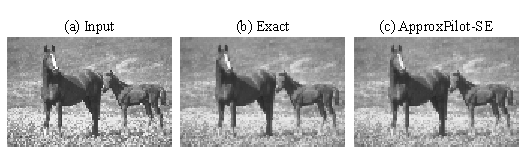
\includegraphics[width=\columnwidth]{figures/case_113016.pdf}
    \caption{Application outputs of the representative high-quality
    DCT76 design. ApproxPilot-SE retains 99.68\% of the
    mean Exact-design SSIM while simultaneously reducing Area, Power,
    and Delay.}
    \label{fig:dct_case}
\end{figure}

Fig.~\ref{fig:dct_case} provides a qualitative comparison of
the corresponding application outputs. The ApproxPilot-SE
output remains visually close to the Exact result while achieving
the PPA reductions reported in Table~\ref{tab:dct_case}.
Together with the verified hypervolume results, this example
shows that the final archive provides practical design choices
spanning both system-level hardware efficiency and
application-level quality.

The following experiments analyze the mechanisms that support
these end-to-end results. We first isolate the effect of
co-evolving surrogate updates during DSE, and then examine
surrogate ranking quality and the timing-domain Delay readout.













%Effect of Co-Evolving DSE
\subsection{Effect of Co-Evolving DSE}
\label{sec:coevolving}

The value of co-evolving DSE lies in where the ground-truth evaluation budget is allocated. We compare it with a One-shot variant using the same surrogate architecture, 900 training labels, and 60 validation configurations. One-shot trains on a method-independent sample of 900 configurations before DSE. ApproxPilot-SE starts from a 540/60 training--validation split (9:1) and acquires 90 configurations in each of four feedback rounds, each with 2,000 surrogate search trials. Both workflows then use 15,000 final search trials and verify 100 candidates plus Exact.

\begin{figure}[!t]
    \centering
    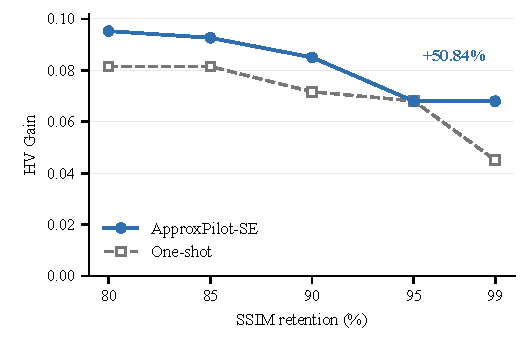
\includegraphics[width=\columnwidth]{figures/coevolving_hv_gain.pdf}
    \caption{Measured HV Gain of ApproxPilot-SE and the aligned One-shot variant under the same target-system training-label budget.}
    \label{fig:coevolving_hv}
\end{figure}

Fig.~\ref{fig:coevolving_hv} compares the measured HV Gain obtained under different SSIM-retention constraints. At 80\%, 85\%, and 90\% retention, ApproxPilot-SE improves HV Gain over One-shot by 16.91\%, 13.69\%, and 18.68\%, respectively. The separation becomes substantially larger under the strictest quality constraint. At 99\% retention, One-shot achieves an HV Gain of 0.045079, whereas ApproxPilot-SE reaches 0.067996, corresponding to a 50.84\% improvement.

Co-evolving DSE directs new system-level measurements toward the Pareto-relevant configurations exposed by search. Updating both surrogates with these measurements lets subsequent rounds refine the same regions, coupling the allocation of training labels to the optimization objective.

At 99\% SSIM retention, the feasible designs must preserve output quality close to Exact. ApproxPilot-SE retains an HV Gain of approximately 0.068 in this region, showing that search-guided label acquisition yields useful PPA tradeoffs under a stringent quality constraint.












%Surrogate Ranking under Limited Labels
%Surrogate Ranking Quality
\subsection{Surrogate Ranking Quality}
\label{sec:surrogate_ranking}

Pareto selection depends on rankings across Area, Power, Delay,
and SSIM. We compare their Spearman correlations at 180, 540,
and 900 training configurations using a common 60-configuration
validation set.

\begin{table}[t]
\centering
\caption{Spearman ranking correlation on the DCT76 validation set.}
\label{tab:surrogate_ranking}
\footnotesize
\setlength{\tabcolsep}{3pt}
\renewcommand{\arraystretch}{1.08}

\begin{tabular*}{\columnwidth}
{@{\extracolsep{\fill}} c l c c c c c @{}}
\toprule
\textbf{Labels} &
\textbf{Method} &
\textbf{A} &
\textbf{P} &
\textbf{D} &
\textbf{Q} &
\textbf{Min.} \\
\midrule

\multirow{3}{*}{180}
& ApproxPilot
& 0.898 & 0.813 & 0.860 & 0.831 & 0.813 \\
& ApproxGNN
& 0.069 & 0.119 & 0.712 & 0.757 & 0.069 \\
& ApproxPilot-SE
& \textbf{0.913}
& \textbf{0.884}
& \textbf{0.866}
& \textbf{0.926}
& \textbf{0.866} \\

\addlinespace[2pt]

\multirow{3}{*}{540}
& ApproxPilot
& 0.920 & 0.850 & 0.885 & 0.900 & 0.850 \\
& ApproxGNN
& 0.168 & 0.156 & 0.701 & 0.867 & 0.156 \\
& ApproxPilot-SE
& \textbf{0.938}
& \textbf{0.908}
& \textbf{0.888}
& \textbf{0.929}
& \textbf{0.888} \\

\addlinespace[2pt]

\multirow{3}{*}{900}
& ApproxPilot
& \textbf{0.963}
& 0.881 & 0.896 & 0.912 & 0.881 \\
& ApproxGNN
& 0.162 & 0.601 & 0.714 & 0.893 & 0.162 \\
& ApproxPilot-SE
& 0.956
& \textbf{0.941}
& \textbf{0.920}
& \textbf{0.949}
& \textbf{0.920} \\

\bottomrule
\end{tabular*}
\par\smallskip
\raggedright A/P/D/Q: Area/Power/Delay/SSIM; Min.: lowest correlation across the four objectives. Bold denotes the highest value at each training size.
\end{table}

With 180 target-system labels, ApproxPilot-SE achieves Spearman
correlations of 0.9126, 0.8835, 0.8664, and 0.9255 for Area,
Power, Delay, and SSIM, respectively, with a minimum correlation
of 0.8664 across all four objectives. At 540 labels,
the corresponding correlations increase to 0.9375, 0.9079,
0.8876, and 0.9290.

At 900 labels, ApproxPilot-SE reaches 0.9557, 0.9412, 0.9202,
and 0.9487 across the four objectives, with a minimum correlation
of 0.9202 and the highest correlations on Power, Delay, and SSIM.

ApproxPilot-SE provides balanced ranking quality across all four
DSE objectives. This property supports Pareto selection, which
compares configurations jointly by hardware cost and output quality.

\begin{figure*}[t]
    \centering
    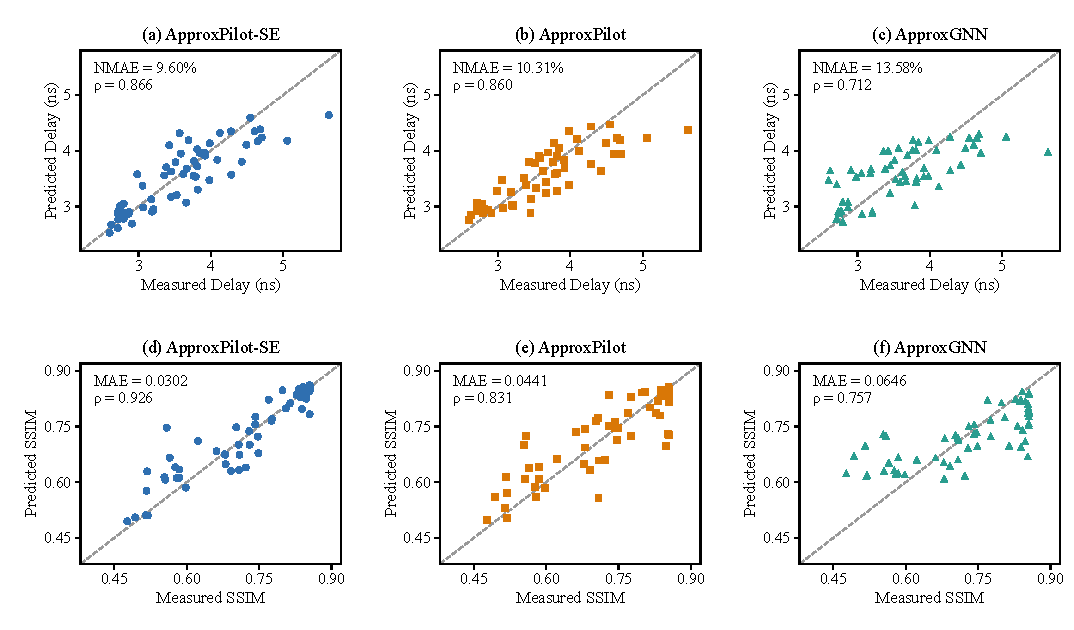
\includegraphics[width=\textwidth]{figures/pred_vs_truth_dct76.pdf}
    \caption{Prediction-versus-ground-truth comparison on DCT76
    with 180 training configurations and 60 validation configurations. The top row shows Delay
    prediction and the bottom row shows SSIM prediction for
    ApproxPilot-SE, ApproxPilot, and ApproxGNN.}
    \label{fig:pred_vs_truth}
\end{figure*}

Fig.~\ref{fig:pred_vs_truth} visualizes Delay and SSIM predictions
under the 180-label setting. Delay NMAE is MAE divided by Exact Delay.
For Delay, ApproxPilot-SE achieves an NMAE of 9.60\% and a
Spearman correlation of 0.866, compared with 10.31\% and 0.860
for ApproxPilot, and 13.58\% and 0.712 for ApproxGNN.
For SSIM, ApproxPilot-SE achieves an MAE of 0.0302 and a
Spearman correlation of 0.926, outperforming ApproxPilot
(0.0441, 0.831) and ApproxGNN (0.0646, 0.757).

The close agreement with measured Delay and SSIM in
Fig.~\ref{fig:pred_vs_truth}, together with the Area and Power
correlations in Table~\ref{tab:surrogate_ranking}, supports the
surrogate ensemble's ability to rank candidate designs with
180 target-system training labels.


















%Timing-Domain Delay Modeling
\subsection{Timing-Domain Delay Modeling}
\label{sec:delay_ablation}

The Delay objective differs from Area and Power because it is
strongly affected by the ordering and interaction of operations
along combinational paths. To evaluate whether the proposed
timing-domain path aggregation contributes useful structural
information beyond a conventional graph-level readout, we compare
it with a Global Max variant. The two models use the same graph
encoder, training data, optimization settings, and Delay targets;
the only difference is the readout used to construct the
configuration-level representation for Delay prediction.

The evaluation set is formed by the union of the final candidates
generated by ApproxPilot-SE, ApproxPilot, ApproxGNN, and the aligned
One-shot workflow. After removing the Exact design and duplicate
configurations, the set contains 400 configurations with measured
system-level Delay. Both variants use 900 training and 60 validation
configurations with paired seeds 101, 202, and 303. The mean and sample standard
deviation are reported in Table~\ref{tab:delay_ablation}.

\begin{table}[t]
\centering
\caption{Ablation of the Delay readout on DCT76. Mean $\pm$ sample standard deviation over three paired seeds.}
\label{tab:delay_ablation}
\footnotesize
\setlength{\tabcolsep}{4pt}
\renewcommand{\arraystretch}{1.08}

\begin{tabular*}{\columnwidth}{@{\extracolsep{\fill}} lcc @{}}
\toprule
\textbf{Metric}
& \textbf{Global Max}
& \textbf{Timing-Domain Path} \\
\midrule
MAE (ns)$\downarrow$
& $0.2095 \pm 0.0102$
& $\mathbf{0.1939 \pm 0.0022}$
\\
Spearman $\rho$$\uparrow$
& $0.7965 \pm 0.0206$
& $\mathbf{0.8217 \pm 0.0228}$
\\
Pairwise Acc. (\%)$\uparrow$
& $80.37 \pm 0.88$
& $\mathbf{81.67 \pm 1.19}$ \\
\bottomrule
\end{tabular*}

\end{table}

The timing-domain path readout improves all three Delay metrics.
Its MAE decreases from 0.2095~ns to 0.1939~ns, corresponding to
a 7.45\% reduction. At the same time, Spearman correlation
increases from 0.7965 to 0.8217, indicating a better ranking of
candidate configurations by measured Delay. Pairwise ranking
accuracy also improves from 80.37\% to 81.67\%.

These results are consistent with the role of the proposed readout
in Section~\ref{sec:method}. Global Max pooling treats node
representations as an unordered set and retains only the strongest
response in each feature dimension. In contrast, timing-domain
path aggregation propagates encoded node states along directed RTL
dependencies before the final aggregation. The resulting
representation therefore preserves information about upstream
operation sequences and competing paths, which is directly
relevant to configuration-level Delay.

The readout thus improves both Delay estimates and the ordering
of candidate designs used by multiobjective search.

\section{Conclusion}
\label{sec:conclusion}

This paper presented ApproxPilot-SE, a co-evolving surrogate-assisted
DSE framework for approximate accelerators. Search-selected
configurations provide new PPA and QoR measurements that update both
surrogates before the next DSE round. This feedback directs the
available training-label budget toward Pareto-relevant regions
of the legal approximation space.

The experimental results show that this interaction between surrogate
learning and search improves the quality of the final verified design
set. On DCT76, ApproxPilot-SE achieves a verified 3-D PPA HV Gain of
0.085054 at 90\% SSIM retention, compared with 0.023273 for the
stronger baseline, and retains an HV Gain of 0.067996 at 99\%
retention. Under the same 900-label target-system training budget,
co-evolving optimization improves verified HV Gain over an aligned
one-shot workflow by up to 50.84\%. The timing-domain path readout
further reduces Delay MAE by 7.45\% relative to global max pooling
while improving both Spearman correlation and pairwise ranking
accuracy.

The final verified archive also contains high-quality configurations
that simultaneously improve multiple hardware objectives while
remaining close to Exact output quality. A representative DCT76
design retains 99.68\% of the Exact-design SSIM while reducing Area,
Power, and Delay by 19.73\%, 20.50\%, and 12.71\%, respectively.
These results demonstrate the value of coupling surrogate updates
with search-guided system-level evaluation for high-quality
approximate-accelerator design.


\FloatBarrier
\bibliographystyle{IEEEtran}
\bibliography{references}
\end{document}
